%======================================================================
% Type the following fields to automatically appear in the right places
%======================================================================
\newcommand{\thesisauthor}{Wail Gueaieb}
\newcommand{\thesistitlecoverpage}{University of Ottawa's Unofficial E-Thesis \LaTeX Template}
\newcommand{\thesisdegree}{Master of Applied Science} % possible values are:
                            % Master of Applied Science / Doctor of Philosophy
\newcommand{\nameofprogram}{Electrical and Computer Engineering}
\newcommand{\graduationyear}{2021}
%======================================================================




% --------------------- Start of Document Preamble -----------------------

% Specify the document class, default style attributes, and page dimensions
% For hyperlinked PDF, suitable for viewing on a computer, use this:
\documentclass[letterpaper,12pt,titlepage,oneside,final]{book}
% For PDF, suitable for double-sided printing, change the PrintVersion variable below
% to "true" and use this \documentclass line instead of the one above:
%\documentclass[letterpaper,12pt,titlepage,openright,twoside,final]{book}

% the following two packages are necessary for using T1 fonts
\usepackage[T1]{fontenc}
\usepackage[utf8]{inputenc}
% \usepackage[latin1]{inputenc}
% Or whatever. Note that the encoding and the font should match. If T1
% does not look nice, try deleting the line with the fontenc. 


% Some LaTeX commands I define for my own nomenclature.
% If you have to, it's better to change nomenclature once here than in a 
% million places throughout your thesis!
\newcommand{\package}[1]{\textbf{#1}} % package names in bold text
\newcommand{\cmmd}[1]{\textbackslash\texttt{#1}} % command name in tt font 
\newcommand{\href}[1]{#1} % does nothing, but defines the command so the
    % print-optimized version will ignore \href tags (redefined by hyperref pkg).
%\newcommand{\texorpdfstring}[2]{#1} % does nothing, but defines the command
% Anything defined here may be redefined by packages added below...

% This package allows if-then-else control structures.
\usepackage{ifthen}
\newboolean{PrintVersion}
\setboolean{PrintVersion}{false} 
% CHANGE THIS VALUE TO "true" as necessary, to improve printed results for hard copies
% by overriding some options of the hyperref package below.


% Citation packages
\usepackage{cite}  % For better handling of numeric citations
% \usepackage[bibencoding=auto,style=numeric,sorting=nyt,backend=biber]{biblatex}  % to handle utf-8 encoding in bibliography
% \addbibresource{bibliography/thesis_lit_review_resources.bib}
%
\usepackage{bibentry} % Needed for inline bibliographic citation, such as in the "Scholarly Outcome" section
\nobibliography* % Tells bibentry to (re)use the bibliographic data from the standard BibTeX setup \bibliography{...}

% Math packages
\usepackage{amsmath,amssymb,amstext,amsfonts} % Lots of math symbols and environments
\usepackage{mathtools}
\usepackage{array}
\usepackage{siunitx}  % To type units
\sisetup{
  per-mode=symbol,
  input-symbols=\pi,
}
\usepackage{physics}  % Convenient for many mathematical notations
\usepackage{bm}
%
\usepackage{amsthm}  % to create theorem-like environments
\newtheorem{lemma}{Lemma}[chapter]
\newtheorem{theorem}{Theorem}[chapter]
\newtheorem{corollary}{Corollary}[chapter]
\newtheorem{definition}{Definition}[chapter]
\newtheorem{example}{Example}[chapter]
\newtheorem{proposition}{Proposition}[chapter]

% Graphic packages
\usepackage[pdftex]{graphicx} % For including graphics N.B. pdftex graphics driver
% To arrange subfigures within the same figure, it is
% recommended to use the package subcaption instead of
% packages subfig or subfigure, for example.
\usepackage{caption}
\usepackage[list=true,labelformat=simple]{subcaption}
\captionsetup[sub]{skip=2pt}
\renewcommand\thesubfigure{(\alph{subfigure})} % for reference like Figure 2(b)

\graphicspath{% figure paths
  {figures/Inkscape/}
  {Figures/Matlab/}
}

% tikz if needed
\usepackage{tikz}
\usetikzlibrary{positioning}
\tikzset{>=stealth}

% List packages
\usepackage{enumitem}

% Table packages
\usepackage{booktabs}  % Nice looking tables


% Algorithm packages
% It is recommended to use algorithmx, as done below, instead of
% using package algorithm2e, for instance.
\usepackage{algorithm,algpseudocode,float}
\usepackage{setspace}
\renewcommand{\algorithmicrequire}{\textbf{Input:}}
\renewcommand{\algorithmicensure}{\textbf{Output:}}
\algnewcommand{\algorithmicand}{\textbf{and }}
\algnewcommand{\algorithmicor}{\textbf{or }}
\algnewcommand{\algAnd}{\algorithmicand}
\algnewcommand{\algOr}{\algorithmicor}

\makeatletter
\@addtoreset{algorithm}{chapter}% algorithm counter resets every chapter
\makeatother
\renewcommand{\thealgorithm}{\arabic{chapter}.\arabic{algorithm}}



% Feedback notes
\usepackage{xargs} % Use more than one optional parameter in a new commands
\usepackage[colorinlistoftodos,prependcaption,textsize=tiny]{todonotes}
%\newcommand\setuptodonotes{tickmarkheight=1pt}
%
\newcommandx{\unsure}[2][1=]{\todo[linecolor=red,backgroundcolor=red!25,bordercolor=red,#1]{#2}}
\newcommandx{\change}[2][1=]{\todo[linecolor=blue,backgroundcolor=blue!25,bordercolor=blue,#1]{#2}}
\newcommandx{\info}[2][1=]{\todo[linecolor=OliveGreen,backgroundcolor=OliveGreen!25,bordercolor=OliveGreen,#1]{#2}}
\newcommandx{\improvement}[2][1=]{\todo[linecolor=Plum,backgroundcolor=Plum!25,bordercolor=Plum,#1]{#2}}
\newcommandx{\thiswillnotshow}[2][1=]{\todo[disable,#1]{#2}}




% sin added for subsubsections to show up
\setcounter{secnumdepth}{5}
\setcounter{tocdepth}{5}


%=== ADD MORE PACKAGES AS NEEDED. TYPICALLY, hyperref (INCLUDED BELOW)
%=== IS THE LAST PACKAGE TO BE LOADED 


%====================================================

% Hyperlinks make it very easy to navigate an electronic document.
% In addition, this is where you should specify the thesis title
% and author as they appear in the properties of the PDF document.
% Use the "hyperref" package 
% N.B. HYPERREF MUST BE THE LAST PACKAGE LOADED; ADD ADDITIONAL PKGS ABOVE
\usepackage[pdftex,pagebackref=false,pdfa]{hyperref} % with basic options
		% N.B. pagebackref=true provides links back from the References to the body text. This can cause trouble for printing.
\hypersetup{
    plainpages=false,       % needed if Roman numbers in frontpages
    unicode=false,          % non-Latin characters in Acrobat’s bookmarks
    pdftoolbar=true,        % show Acrobat’s toolbar?
    pdfmenubar=true,        % show Acrobat’s menu?
    pdffitwindow=false,     % window fit to page when opened
    pdfstartview={FitH},    % fits the width of the page to the window
    % pdftitle={Thesis Title},    % title: CHANGE THIS TEXT!
    % pdfauthor={Author's Name},    % author: CHANGE THIS TEXT! and uncomment this line
    % pdfsubject={Robotics},  % subject: CHANGE THIS TEXT! and uncomment this line
    % pdfkeywords={Robotics} {machine learning} {control systems}, % list of keywords, and uncomment this line if desired
    pdfnewwindow=true,      % links in new window
    colorlinks=true,        % false: boxed links; true: colored links
    linkcolor=blue,         % color of internal links
    citecolor=green,        % color of links to bibliography
    filecolor=magenta,      % color of file links
    urlcolor=cyan           % color of external links
}
\ifthenelse{\boolean{PrintVersion}}{   % for improved print quality, change some hyperref options
\hypersetup{	% override some previously defined hyperref options
%    colorlinks,%
    citecolor=black,%
    filecolor=black,%
    linkcolor=black,%
    urlcolor=black}
}{} % end of ifthenelse (no else)

\usepackage[noabbrev]{cleveref}  % automatically sort references

% Make document PDF-A compliant (for archiving and long-term preservation)
% https://ruor.uottawa.ca/submit-thesis.jsp
% https://webpages.tuni.fi/latex/pdfa-guide.pdf
\usepackage{colorprofiles}
\usepackage[a-3b,mathxmp]{pdfx}

\usepackage[automake,toc,abbreviations]{glossaries-extra} % Exception to the rule of hyperref being the last add-on package


% Setting up margins and other spaces 
% Setting up the page margins...
% uWaterloo thesis requirements specify a minimum of 1 inch (72pt) margin at the
% top, bottom, and outside page edges and a 1.125 in. (81pt) gutter
% margin (on binding side). While this is not an issue for electronic
% viewing, a PDF may be printed, and so we have the same page layout for
% both printed and electronic versions, we leave the gutter margin in.
% Set margins to minimum permitted by uWaterloo thesis regulations:
% \setlength{\marginparwidth}{0pt} % width of margin notes
\setlength{\marginparwidth}{0.8in} % width of margin notes
% N.B. If margin notes are used, you must adjust \textwidth, \marginparwidth
% and \marginparsep so that the space left between the margin notes and page
% edge is less than 15 mm (0.6 in.)
\setlength{\marginparsep}{0pt} % width of space between body text and margin notes
\setlength{\evensidemargin}{0.125in} % Adds 1/8 in. to binding side of all 
% even-numbered pages when the "twoside" printing option is selected
\setlength{\oddsidemargin}{0.125in} % Adds 1/8 in. to the left of all pages
% when "oneside" printing is selected, and to the left of all odd-numbered
% pages when "twoside" printing is selected
\setlength{\textwidth}{6.375in} % assuming US letter paper (8.5 in. x 11 in.) and 
% side margins as above
\raggedbottom

% The following statement specifies the amount of space between
% paragraphs. Other reasonable specifications are \bigskipamount and \smallskipamount.
\setlength{\parskip}{\medskipamount}

% The following statement controls the line spacing.  The default
% spacing corresponds to good typographic conventions and only slight
% changes (e.g., perhaps "1.2"), if any, should be made.
\renewcommand{\baselinestretch}{1} % this is the default line space setting



 


% By default, each chapter will start on a recto (right-hand side)
% page.  We also force each section of the front pages to start on 
% a recto page by inserting \cleardoublepage commands.
% In many cases, this will require that the verso page be
% blank and, while it should be counted, a page number should not be
% printed.  The following statements ensure a page number is not
% printed on an otherwise blank verso page.
\let\origdoublepage\cleardoublepage
\newcommand{\clearemptydoublepage}{%
  \clearpage{\pagestyle{empty}\origdoublepage}}
\let\cleardoublepage\clearemptydoublepage

% Define Glossary terms (This is properly done here, in the preamble. Could be \input{} from a file...)
% Main glossary entries -- definitions of relevant terminology

\newglossaryentry{computer}
{
name=computer,
description={A programmable machine that receives input data,
  stores and manipulates the data, and provides
  formatted output}
}








% List of Abbreviations (abbreviations type is built in to the glossaries-extra package)
% \newabbreviation[<options>]{<label>}{<short>}{<long>}

\newabbreviation{aaaaz}{AAAAZ}{American Association of Amature Astronomers and Zoologists}
\newabbreviation{ADP}{ADP}{Approximate Dynamic Programming}
%
\newabbreviation{FIS}{FIS}{Fuzzy Inference System}
%
\newabbreviation{LMS}{LMS}{Least Mean Squares}
\newabbreviation{LTSM}{LTSM}{Long Short-term Memory}
%
\newabbreviation{RL}{RL}{Reinforcement Learning}
\newabbreviation{RLS}{RLS}{Recursive Least Squares}
%
\newabbreviation{TD}{TD}{Temporal Difference}
\newabbreviation{TS}{TS}{Takagi-Sugeno}











% Nomenclature glossary entries -- New definitions, or unusual terminology
\newglossary*{nomenclature}{Nomenclature}

\newglossaryentry{dingledorf}
{
type=nomenclature,
name=dingledorf,
description={A person of supposed average intelligence who makes incredibly brainless misjudgments}
}










% List of Symbols
\newglossary*{symbols}{List of Symbols}
%
\newglossaryentry{rvec}
{
name={$\mathbf{v}$},
sort={label},
type=symbols,
description={Random vector: a location in n-dimensional Cartesian space, where each dimensional component is determined by a random process}
}
%
%
%
\newglossaryentry{C}
{
name={\ensuremath{\mathcal{C}}},
sort={label},
type=symbols,
description={Configuration space}
}
%
\newglossaryentry{C-space}
{
name={\ensuremath{\mathcal{C}\text{-space}}},
sort={label},
type=symbols,
description={Configuration space}
}
%
\newglossaryentry{C-free}
{
name={\ensuremath{\mathcal{C}^{\text{free}}}},
sort={label},
type=symbols,
description={Configuration space free of constraints/obstacles}
}
%
\newglossaryentry{P}
{
name={\ensuremath{\mathcal{P}}},
sort={label},
type=symbols,
description={Path planning space}
}
%
\newglossaryentry{P-constraint}
{
name={\ensuremath{\mathcal{P}^{\text{constraint}}}},
sort={label},
type=symbols,
description={Path planning space corresponding to constraints (including obstacles)}
}
%
\newglossaryentry{P-free}
{
name={\ensuremath{\mathcal{P}^{\text{free}}}},
sort={label},
type=symbols,
description={$\equiv \mathcal{P} \setminus \mathcal{P}^{\text{constraint}}$ Path planning space free of constraints/obstacles}
}
%
\newglossaryentry{p-goal}
{
name={\ensuremath{\textbf{p}^{\text{goal}}}},
sort={label},
type=symbols,
description={Destination point}
}
%
\newglossaryentry{p-start}
{
name={\ensuremath{\textbf{p}^{\text{start}}}},
sort={label},
type=symbols,
description={Starting point}
}
%
\newglossaryentry{W}
{
name={\ensuremath{\mathcal{W}}},
sort={label},
type=symbols,
description={Workspace}
}





 
\makeglossaries

%======================================================================
%   L O G I C A L    D O C U M E N T -- the content of your thesis
%======================================================================
\begin{document}

% For a large document, it is a good idea to divide your thesis
% into several files, each one containing one chapter.
% To illustrate this idea, the "front pages" (i.e., title page,
% declaration, borrowers' page, abstract, acknowledgements,
% dedication, table of contents, list of tables, list of figures,
% nomenclature) are contained within the file "uo-ethesis-frontpgs.tex" which is
% included into the document by the following statement.
%----------------------------------------------------------------------
% FRONT MATERIAL
%----------------------------------------------------------------------
% T I T L E   P A G E
% -------------------
% Last updated June 14, 2017, by Stephen Carr, IST-Client Services
% The title page is counted as page `i' but we need to suppress the
% page number. Also, we don't want any headers or footers.
\pagestyle{empty}
\pagenumbering{roman}

% F R O N T   P A G E
% -------------------------------

% The contents of the title page are specified in the "titlepage"
% environment.
\begin{titlepage}
        \begin{center}
        \vspace*{1.0cm}

        \Huge
        {\bf \thesistitlecoverpage}
		
        \vspace*{1.0cm}

        \normalsize
        by \\

        \vspace*{1.0cm}

        \Large
        \thesisauthor \\

        \vspace*{3.0cm}

        \normalsize
        Thesis submitted to the University of Ottawa \\ 
        in partial fulfillment of the requirements for the degree of \\
        \thesisdegree \\
        in \\
        \nameofprogram \\
        

        \vspace*{3.0cm}

        \copyright\ {\thesisauthor}, Ottawa, Canada, \graduationyear \\
        \end{center}
\end{titlepage}



% The rest of the front pages should contain no headers and be numbered using Roman numerals starting with `ii'
\pagestyle{plain}
\setcounter{page}{2}

\cleardoublepage % Ends the current page and causes all figures and tables that have so far appeared in the input to be printed.
% In a two-sided printing style, it also makes the next page a right-hand (odd-numbered) page, producing a blank page if necessary.


% E X A M I N I N G   C O M M I T T E E
% -------------------------------

% Remove or comment out the lines below to remove this page
\begin{center}\textbf{Examining Committee}\end{center}
\noindent
The following served on the Examining Committee for this thesis.
\bigskip

\noindent
\begin{tabbing}
  Internal Member(s): \=  \kill % using longest text to define tab length
  External Member: \>  Firstname Lastname\\ % Only required for Ph.D. theses
  \> Professor, Department of Modern Arts\\
  \> University of Southville\\
\end{tabbing} 
\bigskip

\noindent
\begin{tabbing}
  Internal Member(s): \=  \kill % using longest text to define tab length
  Carleton Member: \> Firstname Lastname\\
  \> Associate Professor, Department of Electronics\\
  \> Carleton Univeristy\\
\end{tabbing}
\bigskip

\noindent
\begin{tabbing}
  Internal Member(s): \=  \kill % using longest text to define tab length
  Internal Member(s): \> Firstname Lastname\\
  \> Associate Professor, Department of Mechanical Engineering\\
  \> University of Ottawa\\
  \\
  \> Firstname Lastname\\
  \> Professor, School of Electrical Engineering \& Computer Science\\
  \> University of Ottawa\\
\end{tabbing}
\bigskip

\noindent
\begin{tabbing}
  Internal Member(s): \=  \kill % using longest text to define tab length
  Supervisor(s): \> Wail Gueaieb \\
  \> Professor, School of Electrical Engineering \& Computer Science\\
  \> University of Ottawa \\
\end{tabbing}
\bigskip







\cleardoublepage

% D E C L A R A T I O N   P A G E
% -------------------------------

\begin{center}\textbf{Declaration of Authorship}\end{center}
\noindent
I hereby certify that this thesis is entirely my own original work except where otherwise indicated. I am aware of the University of Ottawa regulations concerning plagiarism, including those regarding consequent disciplinary actions. Any use of the works of any other author, in any form, is properly acknowledged at their point of use.




\cleardoublepage

% A B S T R A C T
% ---------------

\begin{center}\textbf{Abstract}\end{center}
This is the abstract. 

Vulputate minim vel consequat praesent at vel iusto et, ex delenit, esse euismod luptatum augue ut sit et eu vel augue autem feugiat, quis ad dolore. Nulla vel, laoreet lobortis te commodo elit qui aliquam enim ex iriure ea ullamcorper nostrud lorem, lorem laoreet eu ex ut vel in zzril wisi quis. Nisl in autem praesent dignissim, sit vel aliquam at te, vero dolor molestie consequat.

Tation iriure sed wisi feugait odio dolore illum duis in accumsan velit illum consequat consequat ipsum molestie duis duis ut ullamcorper. Duis exerci odio blandit vero dolore eros odio amet et nisl in nostrud consequat iusto eum suscipit autem vero. Iusto dolore exerci, ut erat ex, magna in facilisis duis amet feugait augue accumsan zzril delenit aliquip dignissim at. Nisl molestie nibh, vulputate feugait nibh luptatum ea delenit nostrud dolore minim veniam odio volutpat delenit nulla accumsan eum vero ullamcorper eum. Augue velit veniam, dolor, exerci ea feugiat nulla molestie, veniam nonummy nulla dolore tincidunt, consectetuer dolore nulla ipsum commodo.

At nostrud lorem, lorem laoreet eu ex ut vel in zzril wisi. Suscipit consequat in autem praesent dignissim, sit vel aliquam at te, vero dolor molestie consequat eros tation facilisi diam dolor. Odio luptatum dolor in facilisis et facilisi et adipiscing suscipit eu iusto praesent enim, euismod consectetuer feugait duis. Odio veniam et iriure ad qui nonummy aliquip at qui augue quis vel diam, nulla. Autem exerci tation iusto, hendrerit et, tation esse consequat ut velit te dignissim eu esse eros facilisis lobortis, lobortis hendrerit esse dignissim nisl. Nibh nulla minim vel consequat praesent at vel iusto et, ex delenit, esse euismod luptatum.

Ut eum vero ullamcorper eum ad velit veniam, dolor, exerci ea feugiat nulla molestie, veniam nonummy nulla. Elit tincidunt, consectetuer dolore nulla ipsum commodo, ut, at qui blandit suscipit accumsan feugiat vel praesent. In dolor, ea elit suscipit nisl blandit hendrerit zzril. Sit enim, et dolore blandit illum enim duis feugiat velit consequat iriure sed wisi feugait odio dolore illum duis. Et accumsan velit illum consequat consequat ipsum molestie duis duis ut ullamcorper nulla exerci odio blandit vero dolore eros odio amet et.

In augue quis vel diam, nulla dolore exerci tation iusto, hendrerit et, tation esse consequat ut velit. Duis dignissim eu esse eros facilisis lobortis, lobortis hendrerit esse dignissim nisl illum nulla minim vel consequat praesent at vel iusto et, ex delenit, esse euismod. Nulla augue ut sit et eu vel augue autem feugiat, quis ad dolore te vel, laoreet lobortis te commodo elit qui aliquam enim ex iriure. Ut ullamcorper nostrud lorem, lorem laoreet eu ex ut vel in zzril wisi quis consequat in autem praesent dignissim, sit vel. Dolore at te, vero dolor molestie consequat eros tation facilisi diam. Feugait augue luptatum dolor in facilisis et facilisi et adipiscing suscipit eu iusto praesent enim, euismod consectetuer feugait duis vulputate veniam et.

Ad eros odio amet et nisl in nostrud consequat iusto eum suscipit autem vero enim dolore exerci, ut. Esse ex, magna in facilisis duis amet feugait augue accumsan zzril. Lobortis aliquip dignissim at, in molestie nibh, vulputate feugait nibh luptatum ea delenit nostrud dolore minim veniam odio. Euismod delenit nulla accumsan eum vero ullamcorper eum ad velit veniam. Quis, exerci ea feugiat nulla molestie, veniam nonummy nulla. Elit tincidunt, consectetuer dolore nulla ipsum commodo, ut, at qui blandit suscipit accumsan feugiat vel praesent.

Dolor zzril wisi quis consequat in autem praesent dignissim, sit vel aliquam at te, vero. Duis molestie consequat eros tation facilisi diam dolor augue. Dolore dolor in facilisis et facilisi et adipiscing suscipit eu iusto praesent enim, euismod consectetuer feugait duis vulputate.


\cleardoublepage

% A C K N O W L E D G E M E N T S
% -------------------------------

\begin{center}\textbf{Acknowledgements}\end{center}
All the credit goes to the University of Waterloo. This is mainly a repackaging of their thesis template. 

\cleardoublepage

% D E D I C A T I O N
% -------------------

%\begin{center}\textbf{Dedication}\end{center}
%This is dedicated to the one I love.

\cleardoublepage

% T A B L E   O F   C O N T E N T S
% ---------------------------------
\renewcommand\contentsname{Table of Contents}
\tableofcontents
\cleardoublepage
\phantomsection    % allows hyperref to link to the correct page

% L I S T   O F   T A B L E S
% ---------------------------
\addcontentsline{toc}{chapter}{List of Tables}
\listoftables
\cleardoublepage
\phantomsection		% allows hyperref to link to the correct page

% L I S T   O F   F I G U R E S
% -----------------------------
\addcontentsline{toc}{chapter}{List of Figures}
\listoffigures
\cleardoublepage
\phantomsection		% allows hyperref to link to the correct page

% GLOSSARIES (Lists of definitions, abbreviations, symbols, etc. provided by the glossaries-extra package)
% -----------------------------
\printglossaries
\cleardoublepage
\phantomsection		% allows hyperref to link to the correct page

% Change page numbering back to Arabic numerals
\pagenumbering{arabic}



% Insert list of to do's if needed
% \listoftodos

%----------------------------------------------------------------------
% MAIN BODY
%----------------------------------------------------------------------
% Because this is a short document, and to reduce the number of files
% needed for this template, the chapters are not separate
% documents as suggested above, but you get the idea. If they were
% separate documents, they would each start with the \chapter command, i.e, 
% do not contain \documentclass or \begin{document} and \end{document} commands.
%======================================================================
%======================================================================
\chapter{Introduction}
%======================================================================
In the beginning, there was $\pi$:

\begin{equation}
   e^{\pi i} + 1 = 0  \label{eqn_pi}
\end{equation}
A \gls{computer} could compute $\pi$ all day long. In fact, subsets of digits of $\pi$'s decimal approximation would make a good source for psuedo-random vectors, \gls{rvec} . 

%----------------------------------------------------------------------
\section{State of the Art}
%----------------------------------------------------------------------

See equation~\eqref{eqn_pi} on page \pageref{eqn_pi}.\footnote{A famous equation.}

\section{Some Meaningless Stuff}

The credo of the \gls{aaaaz} was, for several years, several paragraphs of gibberish, until the \gls{dingledorf} responsible for the \gls{aaaaz} Web site realized his mistake:

"Velit dolor illum facilisis zzril ipsum, augue odio, accumsan ea augue molestie lobortis zzril laoreet ex ad, adipiscing nulla. Veniam dolore, vel te in dolor te, feugait dolore ex vel erat duis nostrud diam commodo ad eu in consequat esse in ut wisi. Consectetuer dolore feugiat wisi eum dignissim tincidunt vel, nostrud, at vulputate eum euismod, diam minim eros consequat lorem aliquam et ad. Feugait illum sit suscipit ut, tation in dolore euismod et iusto nulla amet wisi odio quis nisl feugiat adipiscing luptatum minim nisl, quis, erat, dolore. Elit quis sit dolor veniam blandit ullamcorper ex, vero nonummy, duis exerci delenit ullamcorper at feugiat ullamcorper, ullamcorper elit vulputate iusto esse luptatum duis autem. Nulla nulla qui, te praesent et at nisl ut in consequat blandit vel augue ut.

Illum suscipit delenit commodo augue exerci magna veniam hendrerit dignissim duis ut feugait amet dolor dolor suscipit iriure veniam. Vel quis enim vulputate nulla facilisis volutpat vel in, suscipit facilisis dolore ut veniam, duis facilisi wisi nulla aliquip vero praesent nibh molestie consectetuer nulla. Wisi nibh exerci hendrerit consequat, nostrud lobortis ut praesent dignissim tincidunt enim eum accumsan. Lorem, nonummy duis iriure autem feugait praesent, duis, accumsan tation enim facilisi qui te dolore magna velit, iusto esse eu, zzril. Feugiat enim zzril, te vel illum, lobortis ut tation, elit luptatum ipsum, aliquam dolor sed. Ex consectetuer aliquip in, tation delenit dignissim accumsan consequat, vero, et ad eu velit ut duis ea ea odio.

Vero qui, te praesent et at nisl ut in consequat blandit vel augue ut dolor illum facilisis zzril ipsum. Exerci odio, accumsan ea augue molestie lobortis zzril laoreet ex ad, adipiscing nulla, et dolore, vel te in dolor te, feugait dolore ex vel erat duis. Ut diam commodo ad eu in consequat esse in ut wisi aliquip dolore feugiat wisi eum dignissim tincidunt vel, nostrud. Ut vulputate eum euismod, diam minim eros consequat lorem aliquam et ad luptatum illum sit suscipit ut, tation in dolore euismod et iusto nulla. Iusto wisi odio quis nisl feugiat adipiscing luptatum minim. Illum, quis, erat, dolore qui quis sit dolor veniam blandit ullamcorper ex, vero nonummy, duis exerci delenit ullamcorper at feugiat. Et, ullamcorper elit vulputate iusto esse luptatum duis autem esse nulla qui.

Praesent dolore et, delenit, laoreet dolore sed eros hendrerit consequat lobortis. Dolor nulla suscipit delenit commodo augue exerci magna veniam hendrerit dignissim duis ut feugait amet. Ad dolor suscipit iriure veniam blandit quis enim vulputate nulla facilisis volutpat vel in. Erat facilisis dolore ut veniam, duis facilisi wisi nulla aliquip vero praesent nibh molestie consectetuer nulla, iriure nibh exerci hendrerit. Vel, nostrud lobortis ut praesent dignissim tincidunt enim eum accumsan ea, nonummy duis. Ad autem feugait praesent, duis, accumsan tation enim facilisi qui te dolore magna velit, iusto esse eu, zzril vel enim zzril, te. Nisl illum, lobortis ut tation, elit luptatum ipsum, aliquam dolor sed minim consectetuer aliquip.

Tation exerci delenit ullamcorper at feugiat ullamcorper, ullamcorper elit vulputate iusto esse luptatum duis autem esse nulla qui. Volutpat praesent et at nisl ut in consequat blandit vel augue ut dolor illum facilisis zzril ipsum, augue odio, accumsan ea augue molestie lobortis zzril laoreet. Ex duis, te velit illum odio, nisl qui consequat aliquip qui blandit hendrerit. Ea dolor nonummy ullamcorper nulla lorem tation laoreet in ea, ullamcorper vel consequat zzril delenit quis dignissim, vulputate tincidunt ut."

%======================================================================
\chapter{Observations}
%======================================================================

This would be a good place for some figures and tables.

Some notes on figures and photographs\ldots

\begin{itemize}
\item A well-prepared PDF should be 
  \begin{enumerate}
    \item Of reasonable size, {\it i.e.} photos cropped and compressed.
    \item Scalable, to allow enlargment of text and drawings. 
  \end{enumerate} 
\item Photos must be bit maps, and so are not scaleable by definition. TIFF and
BMP are uncompressed formats, while JPEG is compressed. Most photos can be
compressed without losing their illustrative value.
\item Drawings that you make should be scalable vector graphics, \emph{not} 
bit maps. Some scalable vector file formats are: EPS, SVG, PNG, WMF. These can
all be converted into PNG or PDF, that pdflatex recognizes. Your drawing 
package probably can export to one of these formats directly. Otherwise, a 
common procedure is to print-to-file through a Postscript printer driver to 
create a PS file, then convert that to EPS (encapsulated PS, which has a 
bounding box to describe its exact size rather than a whole page). 
Programs such as GSView (a Ghostscript GUI) can create both EPS and PDF from PS files.
Appendix~\ref{AppendixA} shows how to generate properly sized Matlab plots and save them as PDF.
\item It's important to crop your photos and draw your figures to the size that
you want to appear in your thesis. Scaling photos with the 
includegraphics command will cause loss of resolution. And scaling down 
drawings may cause any text annotations to become too small.
\end{itemize}
 
For more information on \LaTeX\, see the uWaterloo Skills for the Academic Workplace  \href{https://uwaterloo.ca/information-systems-technology/services/electronic-thesis-preparation-and-submission-support/ethesis-guide/creating-pdf-version-your-thesis/creating-pdf-files-using-latex/latex-ethesis-and-large-documents}{course notes}. 
\footnote{
Note that while it is possible to include hyperlinks to external documents,
it is not wise to do so, since anything you can't control may change over time. 
It \emph{would} be appropriate and necessary to provide external links to 
additional resources for a multimedia ``enhanced'' thesis. 
But also note that if the \package{hyperref} package is not included, 
as for the print-optimized option in this thesis template, any \cmmd{href} 
commands in your logical document are no longer defined.
A work-around employed by this thesis template is to define a dummy \cmmd{href} 
command (which does nothing) in the preamble of the document, 
before the \package{hyperref} package is included. 
The dummy definition is then redifined by the
\package{hyperref} package when it is included.
}

The classic book by Leslie Lamport \cite{lamport.book}, author of \LaTeX , is worth a look too, and the many available add-on packages are described by 
Goossens \textit{et al} \cite{goossens.book}.




Here is an example of how to include figures in \LaTeX. 
\Cref{fig:beam} shows a cantilever beam of circular cross-section
subjected to a point load and a uniformly distributed load, both of
which are uncertain. Note that it is better not to include the
extension of the figure's source file.

\begin{figure}[hbt]
  \centering
  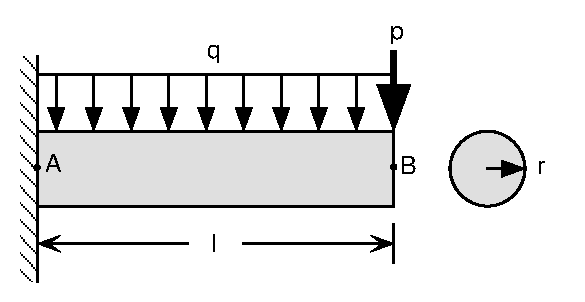
\includegraphics[clip=true]{figures/Inkscape/beam}
  \caption{Cantilever beam}
\label{fig:beam}
\end{figure}


\Cref{tab:prices,tab:team-sheet} show examples of how to add tables in \LaTeX.

\begin{table}[hbt]
  \centering
  \caption{Live stock prices}
  \label{tab:prices}
  \begin{tabular}{llr}  
    \toprule
    \multicolumn{2}{c}{Item} \\
    \cmidrule(r){1-2}
    Animal    & Description & Price (\$) \\
    \midrule
    Gnat      & per gram    & 13.65      \\
              &    each     & 0.01       \\
    Gnu       & stuffed     & 92.50      \\
    Emu       & stuffed     & 33.33      \\
    Armadillo & frozen      & 8.99       \\
    \bottomrule
  \end{tabular}
\end{table}


\begin{table}[hbt]
  \centering
  \caption{Team players}
  \label{tab:team-sheet}
  \begin{tabular}{ll}
    \toprule
    \multicolumn{2}{c}{Team sheet} \\
    \midrule
    GK & Paul Robinson \\
    LB & Lucas Radebe \\
    DC & Michael Duberry \\
    DC & Dominic Matteo \\
    RB & Dider Domi \\
    MC & David Batty \\
    MC & Eirik Bakke \\
    MC & Jody Morris \\
    FW & Jamie McMaster \\
    ST & Alan Smith \\
    ST & Mark Viduka \\
    \bottomrule
  \end{tabular}
\end{table}




Some examples of theorem-like environments. \Cref{def:prime} defines prime numbers. \Cref{cor:vertical-angles} is a consequence of \Cref{thm:one-side-line}.
%
\begin{definition}[Prime numbers]\label{def:prime}
  A prime number is a natural number that is only divisible by itself and 1.
\end{definition}
%
\begin{theorem}[Angles on one side of a line]\label{thm:one-side-line}
  Angles on one side of a straight line always add to \ang{180}.
\end{theorem}
%
\begin{corollary}[Vertical angles]\label{cor:vertical-angles}
  A corollary is a consequence of a theorem. 
  Following on from \Cref{thm:one-side-line} we find that where two lines intersect, opposite angles (also called Vertical Angles) are always equal.
\end{corollary}





%======================================================================
\chapter{Recommendations}
%======================================================================

Every chapter in a thesis should begin with an introduction and end with a conclusion or a summary.


%----------------------------------------------------------------------
\section{Equations}
% ----------------------------------------------------------------------

In general, equations should be unnumbered unless they referred to in the text. Remember not to leave an empty line before or after the equation in \LaTeX\ because that would start a new paragraph.
%
\begin{equation*}
   \mathcal{R} : \mathbb{R} \to \mathbb{R}^1
\end{equation*}
%
Sometimes, it is better to group related equations together as in~\eqref{eq:trigonometry}. You can refer to subequations as~\eqref{eq:trigonometry:cos}, for example. 
%
\begin{subequations}
  \label{eq:trigonometry}
  \begin{gather}
    \sin^2{\theta} + \cos^2{\theta} = 1  \label{eq:trigonometry:sum}\\
    \cos \theta = \frac{1 - \tan^2(\theta/2)}{1 + \tan^2(\theta/2)}   \label{eq:trigonometry:cos}\\
    \sin \theta = \frac{2 \tan(\theta/2)}{1 + \tan^2(\theta/2)}   \label{eq:trigonometry:sin}
  \end{gather}
\end{subequations}




%----------------------------------------------------------------------
\section{Figures}
% ----------------------------------------------------------------------

\Cref{fig:beam} shows one way of inserting a figure. However, it is sometimes useful to group a few figures together, as in \Cref{fig:experiment1}. For that, it is recommended to use package \texttt{subcaption}. It is preferred to other packages, such as \texttt{subfig}, for instance. Note how you can refer to a subfigure too (e.g.,~\Cref{fig:experiment1:states}).

\begin{figure}[htb]
  \centering
  % 
  \subcaptionbox{Reference/measured vertical acceleration%
    \label{fig:experiment1:ref}}%[12em]%
  {%
    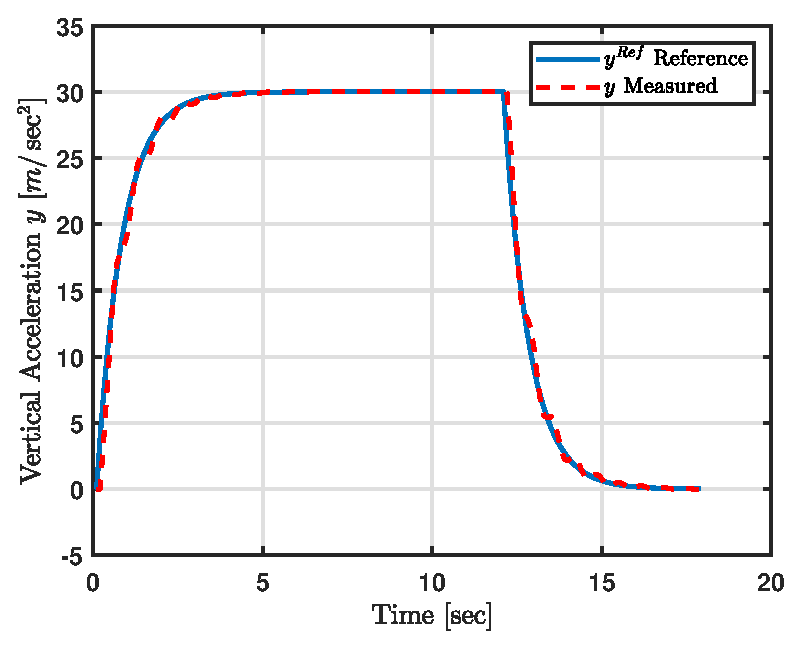
\includegraphics[width=0.32\textwidth]{figures/Matlab/Fig1_1}%
  }
  % 
  \hfill
  %
  \subcaptionbox{Tracking error~$e(t)$%
    \label{fig:experiment1:err}}%[12em]%
  {%
    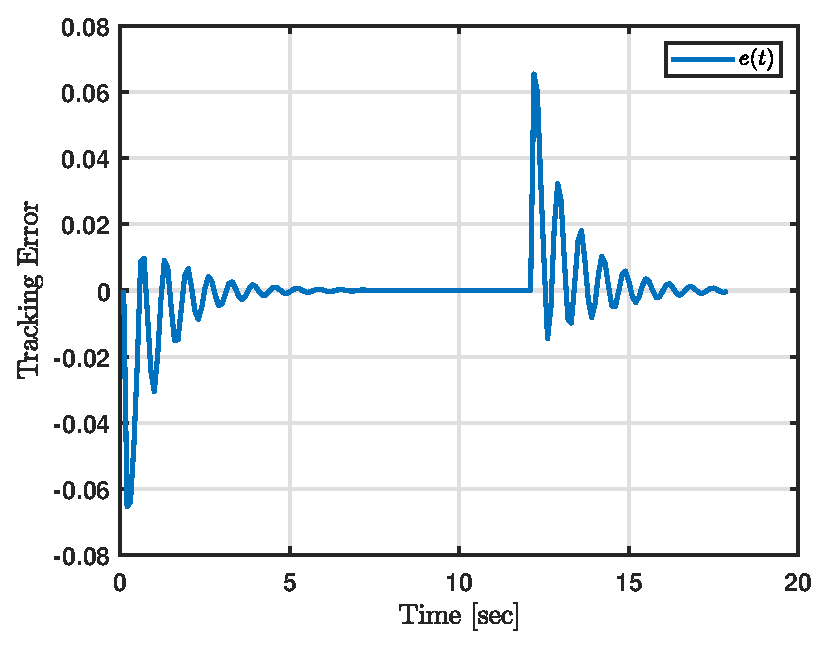
\includegraphics[width=0.32\textwidth]{figures/Matlab/Fig1_5}%
  }
  %
  \hfill
  %
  \subcaptionbox{System states $\alpha(t)$ and~$q(t)$%
    \label{fig:experiment1:states}}%[12em]%
  {%
    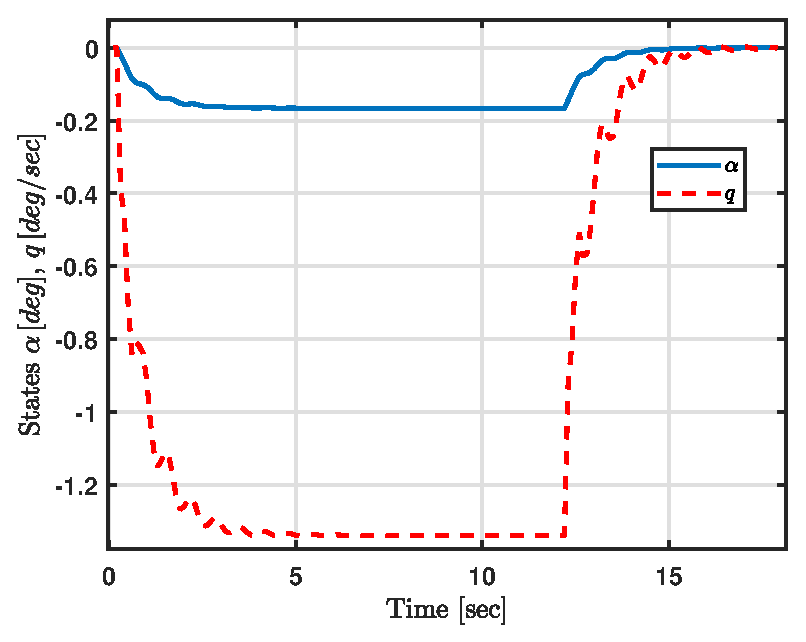
\includegraphics[width=0.32\textwidth]{figures/Matlab/Fig1_2}%
  }
  %
  \\[2ex]
  \mbox{}\hfill
  \subcaptionbox{Elevator deflection~$\bm{u}(t)$%
    \label{fig:experiment1:con}}%[12em]%
  {%
    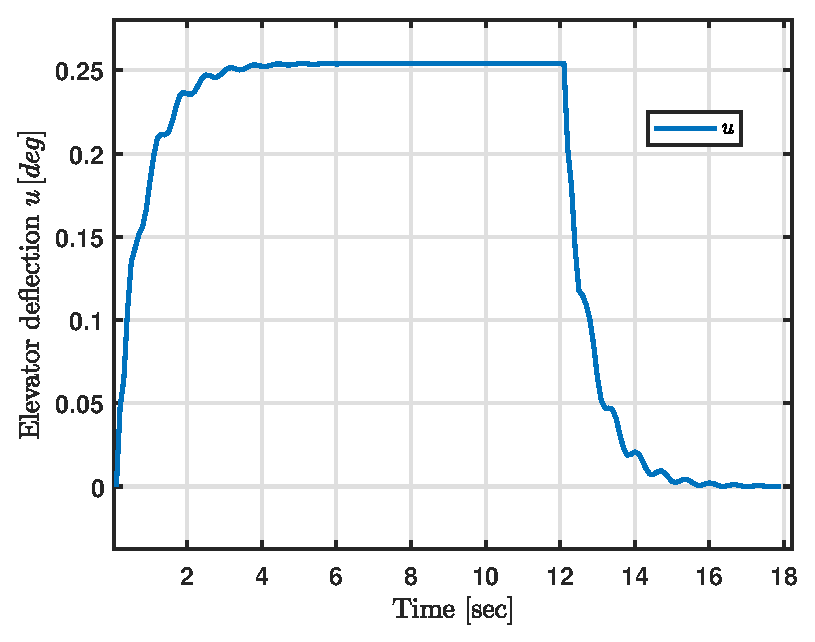
\includegraphics[width=0.32\textwidth]{figures/Matlab/Fig1_3}%
  }
  %
  \hfill
  %
  \subcaptionbox{Control gains~$K(t)$%
    \label{fig:experiment1:act}}%[12em]%
  {%
    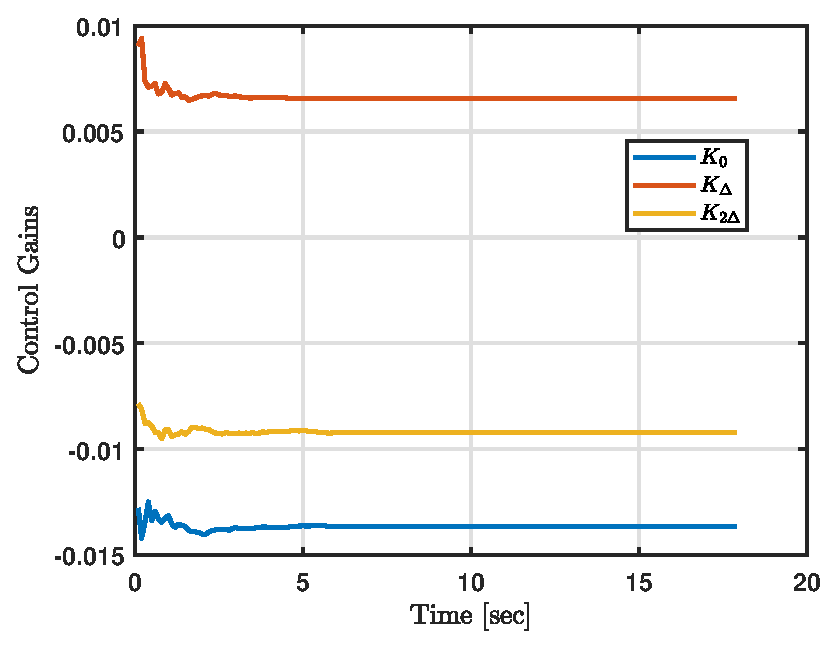
\includegraphics[width=0.32\textwidth]{figures/Matlab/Fig1_4}%
  }
  \hfill\mbox{}
  %
  \caption{Simulation results of test case~1\label{fig:experiment1}} 
\end{figure}





%----------------------------------------------------------------------
\section{Algorithms}
%----------------------------------------------------------------------

\Cref{alg:power} shows an example of how to write algorithms using the \texttt{algorithmicx} package, which is preferred to other packages, such \texttt{algorithmic} and \texttt{algorithm2e}, for example.

\begin{algorithm}[hbt] % or [H]
  \caption{Computing the power of a real number}
  \label{alg:power}
  \begin{algorithmic}[1] % The number tells the line numbering frequency
    \Require
    \Statex $n \geq 0$ \Comment{First input/requirement}
    \Statex $x \in \mathbb{R}$
    \Ensure
    \Statex $y = x^n$
    \Statex % Non-numbered statement
    %
    \State $y \gets 1$
    \State $X \gets x$
    \State $N \gets n$
    \While{$N \neq 0$}
    \If{$N$ is even \algOr $N$ is even}  \Comment{For demonstration purpose}
    \State $X \gets X \times X$
    \State $N \gets \frac{N}{2} $  \Comment{This is a comment}
    \ElsIf{$N$ is odd \algAnd $N$ is odd}
    \State $y \gets y \times X$
    \State $N \gets N - 1$
    \EndIf
    \EndWhile
    %
    \State \Return $y$
  \end{algorithmic}
\end{algorithm}



%----------------------------------------------------------------------
\section{Lists}
%----------------------------------------------------------------------
The default spacing of \LaTeX\ lists can be an eyesore. The package \texttt{enumitem} provides a convenient mechanism to customize them, as illustrated below. Please refer to the package documentation for details.

\begin{itemize}[leftmargin=*, noitemsep]
\item Illum suscipit delenit commodo augue exerci magna veniam hendrerit dignissim duis ut feugait amet dolor dolor suscipit iriure veniam. Vel quis enim vulputate nulla facilisis volutpat vel in, suscipit facilisis dolore ut veniam, duis facilisi wisi nulla aliquip vero praesent nibh molestie consectetuer nulla. Wisi nibh exerci hendrerit consequat, nostrud lobortis ut praesent dignissim tincidunt enim eum accumsan. Lorem, nonummy duis iriure autem feugait praesent, duis, accumsan tation enim facilisi qui te dolore magna velit, iusto esse eu, zzril. Feugiat enim zzril, te vel illum, lobortis ut tation, elit luptatum ipsum, aliquam dolor sed. Ex consectetuer aliquip in, tation delenit dignissim accumsan consequat, vero, et ad eu velit ut duis ea ea odio.
  
\item Vero qui, te praesent et at nisl ut in consequat blandit vel augue ut dolor illum facilisis zzril ipsum. Exerci odio, accumsan ea augue molestie lobortis zzril laoreet ex ad, adipiscing nulla, et dolore, vel te in dolor te, feugait dolore ex vel erat duis. Ut diam commodo ad eu in consequat esse in ut wisi aliquip dolore feugiat wisi eum dignissim tincidunt vel, nostrud. Ut vulputate eum euismod, diam minim eros consequat lorem aliquam et ad luptatum illum sit suscipit ut, tation in dolore euismod et iusto nulla. Iusto wisi odio quis nisl feugiat adipiscing luptatum minim. Illum, quis, erat, dolore qui quis sit dolor veniam blandit ullamcorper ex, vero nonummy, duis exerci delenit ullamcorper at feugiat. Et, ullamcorper elit vulputate iusto esse luptatum duis autem esse nulla qui.

\item Praesent dolore et, delenit, laoreet dolore sed eros hendrerit consequat lobortis. Dolor nulla suscipit delenit commodo augue exerci magna veniam hendrerit dignissim duis ut feugait amet. Ad dolor suscipit iriure veniam blandit quis enim vulputate nulla facilisis volutpat vel in. Erat facilisis dolore ut veniam, duis facilisi wisi nulla aliquip vero praesent nibh molestie consectetuer nulla, iriure nibh exerci hendrerit. Vel, nostrud lobortis ut praesent dignissim tincidunt enim eum accumsan ea, nonummy duis. Ad autem feugait praesent, duis, accumsan tation enim facilisi qui te dolore magna velit, iusto esse eu, zzril vel enim zzril, te. Nisl illum, lobortis ut tation, elit luptatum ipsum, aliquam dolor sed minim consectetuer aliquip.
\end{itemize}

\begin{enumerate}[leftmargin=*, noitemsep]
\item Illum suscipit delenit commodo augue exerci magna veniam hendrerit dignissim duis ut feugait amet dolor dolor suscipit iriure veniam. Vel quis enim vulputate nulla facilisis volutpat vel in, suscipit facilisis dolore ut veniam, duis facilisi wisi nulla aliquip vero praesent nibh molestie consectetuer nulla. Wisi nibh exerci hendrerit consequat, nostrud lobortis ut praesent dignissim tincidunt enim eum accumsan. Lorem, nonummy duis iriure autem feugait praesent, duis, accumsan tation enim facilisi qui te dolore magna velit, iusto esse eu, zzril. Feugiat enim zzril, te vel illum, lobortis ut tation, elit luptatum ipsum, aliquam dolor sed. Ex consectetuer aliquip in, tation delenit dignissim accumsan consequat, vero, et ad eu velit ut duis ea ea odio.
  
\item Vero qui, te praesent et at nisl ut in consequat blandit vel augue ut dolor illum facilisis zzril ipsum. Exerci odio, accumsan ea augue molestie lobortis zzril laoreet ex ad, adipiscing nulla, et dolore, vel te in dolor te, feugait dolore ex vel erat duis. Ut diam commodo ad eu in consequat esse in ut wisi aliquip dolore feugiat wisi eum dignissim tincidunt vel, nostrud. Ut vulputate eum euismod, diam minim eros consequat lorem aliquam et ad luptatum illum sit suscipit ut, tation in dolore euismod et iusto nulla. Iusto wisi odio quis nisl feugiat adipiscing luptatum minim. Illum, quis, erat, dolore qui quis sit dolor veniam blandit ullamcorper ex, vero nonummy, duis exerci delenit ullamcorper at feugiat. Et, ullamcorper elit vulputate iusto esse luptatum duis autem esse nulla qui.

\item Praesent dolore et, delenit, laoreet dolore sed eros hendrerit consequat lobortis. Dolor nulla suscipit delenit commodo augue exerci magna veniam hendrerit dignissim duis ut feugait amet. Ad dolor suscipit iriure veniam blandit quis enim vulputate nulla facilisis volutpat vel in. Erat facilisis dolore ut veniam, duis facilisi wisi nulla aliquip vero praesent nibh molestie consectetuer nulla, iriure nibh exerci hendrerit. Vel, nostrud lobortis ut praesent dignissim tincidunt enim eum accumsan ea, nonummy duis. Ad autem feugait praesent, duis, accumsan tation enim facilisi qui te dolore magna velit, iusto esse eu, zzril vel enim zzril, te. Nisl illum, lobortis ut tation, elit luptatum ipsum, aliquam dolor sed minim consectetuer aliquip.
\end{enumerate}




%----------------------------------------------------------------------
\section{Glossaries}
%----------------------------------------------------------------------
In this template, glossaries are implemented using the package \texttt{glossaries-extra}. Type your glossaries in the file \texttt{glossary.tex}. Either follow the template of the glossary definitions therein or refer to the package documentation.

Here is an example on how to use glossaries. If this is the first time \Gls{FIS} is mentioned in the document, then the full definition is displayed. If it is mentioned again (\Gls{FIS}), then only the abbreviation is shown.




%----------------------------------------------------------------------
\section{Summary}
%----------------------------------------------------------------------
In this chapter, we went through a few recommendations which students may want to keep in mind while typing their theses in \LaTeX.  


%----------------------------------------------------------------------
% END MATERIAL
%----------------------------------------------------------------------

% B I B L I O G R A P H Y
% -----------------------

% The following statement selects the style to use for references.  It controls the sort order of the entries in the bibliography and also the formatting for the in-text labels.
\bibliographystyle{plain}
% This specifies the location of the file containing the bibliographic information.  
% It assumes you're using BibTeX (if not, why not?).
\cleardoublepage % This is needed if the book class is used, to place the anchor in the correct page,
                 % because the bibliography will start on its own page.
                 % Use \clearpage instead if the document class uses the "oneside" argument
\phantomsection  % With hyperref package, enables hyperlinking from the table of contents to bibliography             
% The following statement causes the title "References" to be used for the bibliography section:
\renewcommand*{\bibname}{References} 

% Add the References to the Table of Contents
\addcontentsline{toc}{chapter}{\textbf{References}}

% Commented below to include my own bib file
\bibliography{bibliography/uo-ethesis}
%\printbibliography



% The \appendix statement indicates the beginning of the appendices.
\appendix
% Add a title page before the appendices and a line in the Table of Contents
\chapter*{APPENDICES}
\addcontentsline{toc}{chapter}{APPENDICES}
% %======================================================================
% An appendix
%======================================================================
\chapter[PDF Plots From Matlab]{Matlab Code for Making a PDF Plot}
\label{AppendixA}
% Tip 4: Example of how to get a shorter chapter title for the Table of Contents 
%======================================================================
\section{Using the GUI}
Properties of Matab plots can be adjusted from the plot window via a graphical interface. Under the Desktop menu in the Figure window, select the Property Editor. You may also want to check the Plot Browser and Figure Palette for more tools. To adjust properties of the axes, look under the Edit menu and select Axes Properties.

To set the figure size and to save as PDF or other file formats, click the Export Setup button in the figure Property Editor.

\section{From the Command Line} 
All figure properties can also be manipulated from the command line. Here's an example: 
\begin{verbatim}
x=[0:0.1:pi];
hold on % Plot multiple traces on one figure
plot(x,sin(x))
plot(x,cos(x),'--r')
plot(x,tan(x),'.-g')
title('Some Trig Functions Over 0 to \pi') % Note LaTeX markup!
legend('{\it sin}(x)','{\it cos}(x)','{\it tan}(x)')
hold off
set(gca,'Ylim',[-3 3]) % Adjust Y limits of "current axes"
set(gcf,'Units','inches') % Set figure size units of "current figure"
set(gcf,'Position',[0,0,6,4]) % Set figure width (6 in.) and height (4 in.)
cd n:\thesis\plots % Select where to save
print -dpdf plot.pdf % Save as PDF
\end{verbatim}


\end{document}















